\documentclass[11pt, a4paper]{article}
\usepackage[utf8]{inputenc}
\usepackage[margin=1in]{geometry}
\usepackage{graphicx}
\usepackage{times}
\usepackage{amsmath}
\usepackage{amssymb}
\graphicspath{{./images/}}
\title{Study on B+ Tree}
\author{Riyad-E-Al Muhafiz, 170042036 }
\date{\today}

\begin{document}

\maketitle
\section{Introduction}
\subsection{What is a B+ Tree?}
A B+ Tree is primarily utilized for implementing dynamic indexing on multiple levels. Compared to B- Tree, the B+ Tree stores the data pointers only at the leaf nodes of the Tree, which makes search more process more accurate and faster.
\subsection{Motivation}
\noindent B+ Tree are used to store the large amount of data which can not be stored in the main memory. Due to the fact that, size of main memory is always limited, the internal nodes (keys to access records) of the B+ tree are stored in the main memory whereas, leaf nodes are stored in the secondary memory.
\subsection{History}
\noindent The B tree was first described in the paper Organization and Maintenance of Large Ordered Indices. Acta Informatica 1: 173–189 (1972) by Rudolf Bayer and Edward M. McCreight. There is no single paper introducing the B+ tree concept. Instead, the notion of maintaining all data in leaf nodes is repeatedly brought up as an interesting variant. An early survey of B trees also covering B+ trees is Douglas Comer. Comer notes that the B+ tree was used in IBM's VSAM data access software and he refers to an IBM published article from 1973.
\subsection{B+ tree in real life}
The ReiserFS, NSS, XFS, JFS, ReFS, and BFS filesystems all use this type of tree for metadata indexing; BFS also uses B+ trees for storing directories. NTFS uses B+ trees for directory and security-related metadata indexing.
\section{Problem Formulation}
\noindent In computer science, a B+ tree is a type of tree data structure. It represents sorted data in a way that allows for efficient insertion and removal of elements. It is a dynamic, multilevel index with maximum and minimum bounds on the number of keys in each node. \vspace{0.5cm}

\noindent A B+ tree is a variation on a B-tree. In a B+ tree, in contrast to a B tree, all data are saved in the leaves. Internal nodes contain only keys and tree pointers. All leaves are at the same lowest level. Leaf nodes are also linked together as a linked list to make range queries easy. \vspace{0.5cm}

\noindent The maximum number of keys in a record is called the order of the B+ tree. \vspace{0.5cm}

\noindent The minimum number of keys per record is 1/2 of the maximum number of keys. For example, if the order of a B+ tree is n, each node (except for the root) must have between n/2 and n keys. \vspace{0.5cm}

\noindent The number of keys that may be indexed using a B+ tree is a function of the order of the tree and its height. \vspace{0.5cm}

\noindent For a n-order B+ tree with a height of h: 

\begin{itemize}
    \item maximum number of keys is $n^h$.
    \item minimum number of keys is  $2(n/2)^{h-1}$.
\end{itemize}

\noindent The leaves (the bottom-most index blocks) of the B+ tree are often linked to one another in a linked list; this makes range queries or an (ordered) iteration through the blocks simpler and more efficient (though the aforementioned upper bound can be achieved even without this addition). This does not substantially increase space consumption or maintenance on the tree. This illustrates one of the significant advantages of a B+tree over a B-tree; in a B-tree, since not all keys are present in the leaves, such an ordered linked list cannot be constructed. A B+tree is thus particularly useful as a database system index, where the data typically resides on disk, as it allows the B+tree to actually provide an efficient structure for housing the data itself (this is described in as index structure.

\noindent If a storage system has a block size of B bytes, and the keys to be stored have a size of k, arguably the most efficient B+ tree is one where $b=\frac{B}{k}-1$. Although theoretically the one-off is unnecessary, in practice there is often a little extra space taken up by the index blocks (for example, the linked list references in the leaf blocks). Having an index block which is slightly larger than the storage system's actual block represents a significant performance decrease; therefore erring on the side of caution is preferable.

\noindent If nodes of the B+ tree are organized as arrays of elements, then it may take a considerable time to insert or delete an element as half of the array will need to be shifted on average. To overcome this problem, elements inside a node can be organized in a binary tree or a B+ tree instead of an array.

\noindent B+ trees can also be used for data stored in RAM. In this case a reasonable choice for block size would be the size of processor's cache line.
\noindent Space efficiency of B+ trees can be improved by using some compression techniques. One possibility is to use delta encoding to compress keys stored into each block. For internal blocks, space saving can be achieved by either compressing keys or pointers. For string keys, space can be saved by using the following technique: Normally the $i-th$ entry of an internal block contains the first key of block $i+1$.. Instead of storing the full key, we could store the shortest prefix of the first key of block $i+1$ that is strictly greater (in lexicographic order) than last key of block i. There is also a simple way to compress pointers: if we suppose that some consecutive blocks $ i,i+1,...i+k$ are stored contiguously, then it will suffice to store only a pointer to the first block and the count of consecutive blocks

\section{General Solution}

\subsection{Operations of B+ tree}
There are 3 types of operations we can perform using B+ tree. They are:
\begin{itemize}
    \item Search Operation
    \item Insert Operation
    \item Delete Operation
\end{itemize}

\subsubsection{Search Operation}
In B+ Tree, a search is one of the easiest procedures to execute and get fast and accurate results from it.

The following search algorithm is applicable:

\begin{itemize}
    \item To find the required record, you need to execute the binary search on the available records in the Tree.
    \item In case of an exact match with the search key, the corresponding record is returned to the user.
    \item In case the exact key is not located by the search in the parent, current, or leaf node, then a "not found message" is displayed to the user.
    \item The search process can be re-run for better and more accurate results.
\end{itemize}

\begin{figure}[h]
    \centering
    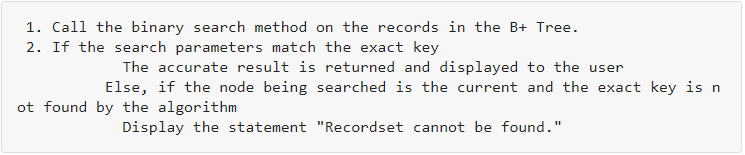
\includegraphics{search.png}
    \caption{Search Operation Algorithm}
    \label{Search}
\end{figure}

\noindent \textbf{Output:}

\noindent The matched record set against the exact key is displayed to the user; otherwise, a failed attempt is shown to the user.

\subsubsection{Insert Operation}

\noindent The following algorithm is applicable for the insert operation:

\begin{itemize}
    \item 50 percent of the elements in the nodes are moved to a new leaf for storage.
    \item The parent of the new Leaf is linked accurately with the minimum key value and a new location in the Tree.
    \item Split the parent node into more locations in case it gets fully utilized.
    \item Now, for better results, the center key is associated with the top-level node of that Leaf.
    \item Until the top-level node is not found, keep on iterating the process explained in the above steps.
\end{itemize}

\begin{figure}[h]
    \centering
    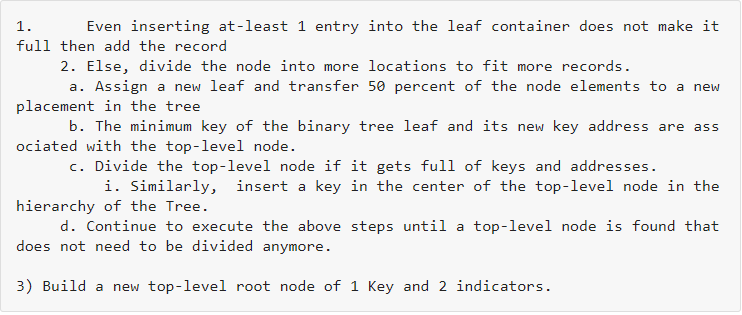
\includegraphics[scale=0.5]{insert.png}
    \caption{Insert Operation Algorithm}
    \label{insert}
\end{figure}



\begin{figure}[h]
    \centering
    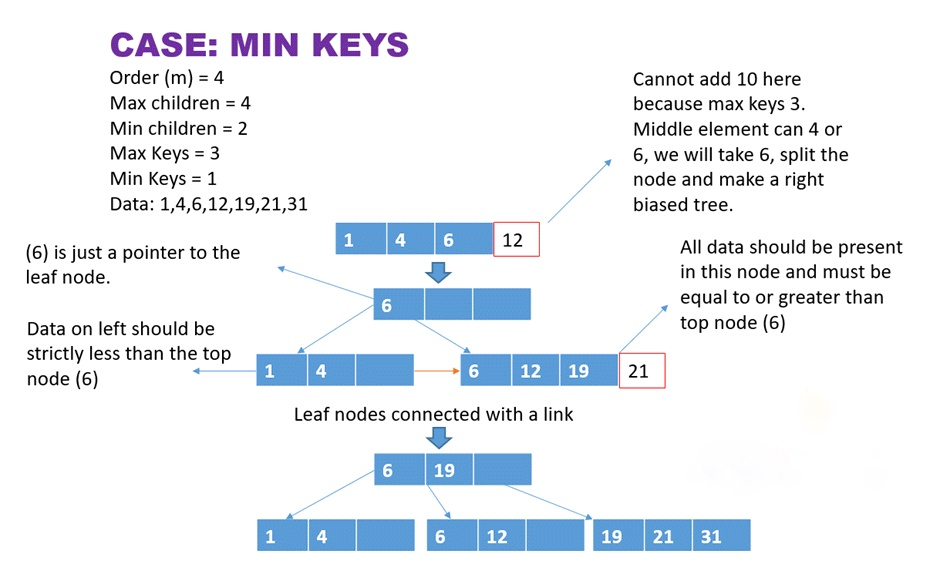
\includegraphics[scale=0.5]{insert1.jpeg}
    \label{insert}
\end{figure}

\noindent The above B+ Tree sample example is explained in the steps below:

\begin{itemize}
    \item Firstly, we have 3 nodes, and the first 3 elements, which are 1, 4, and 6, are added on appropriate locations in the nodes.
    \item The next value in the series of data is 12 that needs to be made part of the Tree.
    \item To achieve this, divide the node, add 6 as a pointer element.
    \item Now, a right-hierarchy of a tree is created, and remaining data values are adjusted accordingly by keeping in mind the applicable rules of equal to or greater than values against the key-value nodes on the right.
\end{itemize}


\subsubsection{Delete Operation}

\noindent The complexity of the delete procedure in the B+ Tree surpasses that of the insert and search functionality.

\noindent The following algorithm is applicable for the insert operation:

\begin{itemize}
    \item Firstly, we need to locate a leaf entry in the Tree that is holding the key and pointer. , delete the leaf entry from the Tree if the Leaf fulfills the exact conditions of record deletion.
    \item In case the leaf node only meets the satisfactory factor of being half full, then the operation is completed; otherwise, the Leaf node has minimum entries and cannot be deleted.
    \item The other linked nodes on the right and left can vacate any entries then move them to the Leaf. If these criteria is not fulfilled, then they should combine the leaf node and its linked node in the tree hierarchy.
    \item Upon merging of leaf node with its neighbors on the right or left, entries of values in the leaf node or linked neighbor pointing to the top-level node are deleted.
\end{itemize}

\begin{figure}[h]
    \centering
    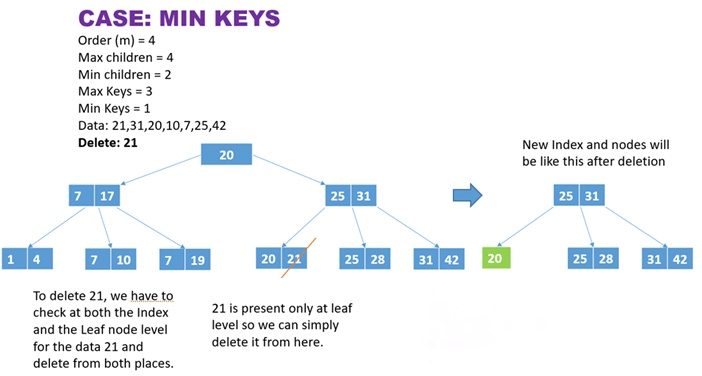
\includegraphics[scale=.5]{del1.jpeg}
    \label{del1}
\end{figure}

\noindent The example above illustrates the procedure to remove an element from the B+ Tree of a specific order.

\begin{itemize}
    \item Firstly, the exact locations of the element to be deleted are identified in the Tree.
    \item Here the element to be deleted can only be accurately identified at the leaf level and not at the index placement. Hence, the element can be deleted without affecting the rules of deletion, which is the value of the bare-minimum key.
    
    \begin{figure}[h]
    \centering
    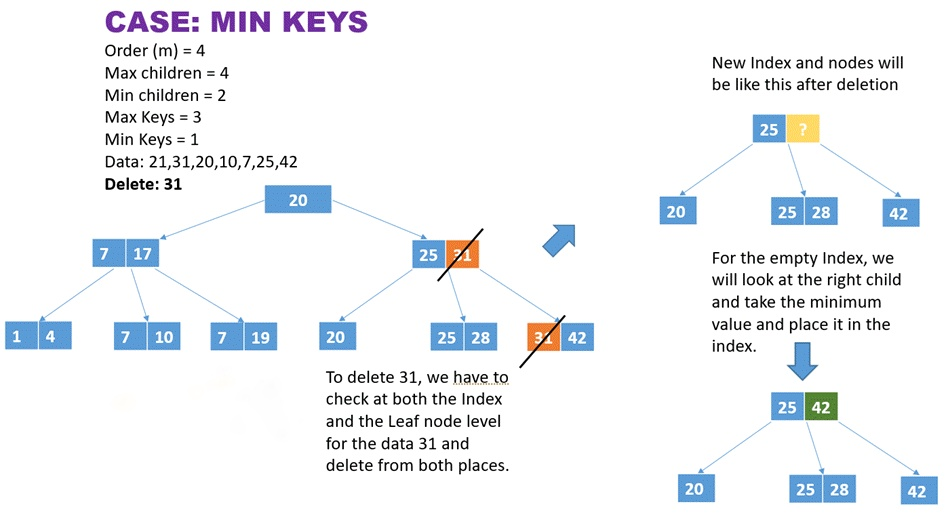
\includegraphics[scale=.5]{del2.jpeg}
    \label{del2}
\end{figure}
    
    \item In the above example, we have to delete 31 from the Tree.
    \item We need to locate the instances of 31 in Index and Leaf.
    \item We can see that 31 is available in both Index and Leaf node level. Hence, we delete it from both instances.
    \item But, we have to fill the index pointing to 42. We will now look at the right child under 25 and take the minimum value and place it as an index. So, 42 being the only value present, it will become the index.
\end{itemize} \vspace{1cm}


\begin{figure}[h]
    \centering
    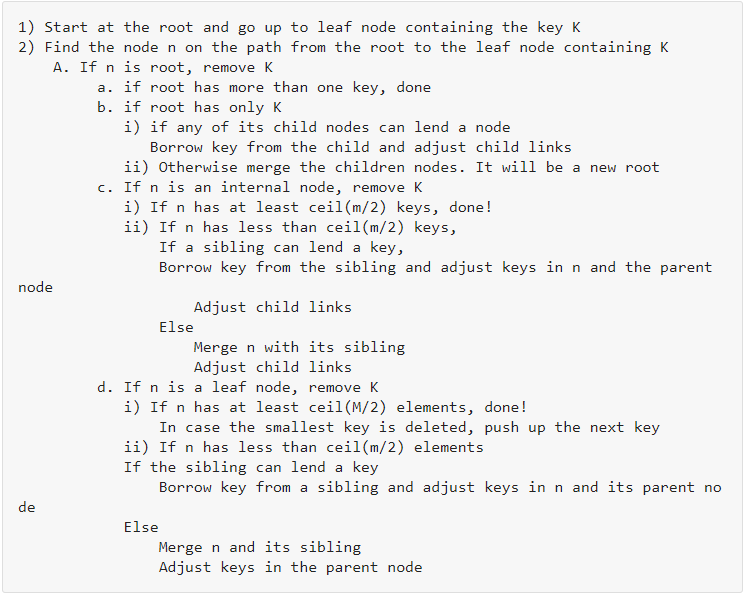
\includegraphics{delete.png}
    \caption{Delete Operation Algorithm}
    \label{delete}
\end{figure}

\noindent \textbf{Output:}

\noindent The Key "K" is deleted, and keys are borrowed from siblings for adjusting values in n and its parent nodes if needed.


\section{Example}

We will see an example of Insertion in B+ tree. 

\begin{itemize}
    \item Each node except root can have a maximum of \textbf{M} children and at least \textbf{ceil(M/2)} children.
    \item Each node can contain a maximum of \textbf{M} – 1 keys and a minimum of \textbf{ceil(M/2) – 1} keys.
    \item The root has at least two children and atleast one search key.
    \item While insertion overflow of the node occurs when it contains more than \textbf{M} – 1 search key values.
\end{itemize}

\noindent Here M is the order of B+ tree. \vspace{0.5cm}

\noindent Steps for insertion in B+ Tree \vspace{0.5cm}

\noindent \textbf{Step 1:} Every element is inserted into a leaf node. So, go to the appropriate leaf node.

\noindent \textbf{Step 2:} Insert the key into the leaf node in increasing order only if there is no overflow. If there is an overflow go ahead with the following steps mentioned below to deal with overflow while maintaining the B+ Tree properties.

\noindent \textbf{Case 1:}

\begin{enumerate}
  \item Split the leaf node into two nodes.
  \item First node contains ceil((m-1)/2) values. environment.
  \item Second node contains the remaining values.
  \item Copy the smallest search key value from second node to the parent node.(Right biased)
\end{enumerate}

\noindent Below is the illustration of inserting 8 into B+ Tree of order of 5:

\begin{figure}[h]
    \centering
    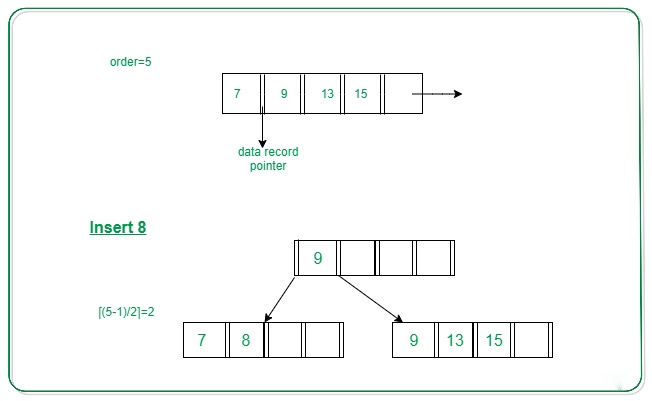
\includegraphics[scale=0.4]{in1.jpeg}
    \label{in1}
\end{figure}

\noindent \textbf{Case 2:}

\begin{enumerate}
  \item Split the leaf node into two nodes.
  \item First node contains ceil(m/2)-1 values.
  \item Move the smallest among remaining to the parent.
  \item Second node contains the remaining keys.
\end{enumerate}

\noindent Below is the illustration of inserting 15 into B+ Tree of order of 5:

\begin{figure}[h]
    \centering
    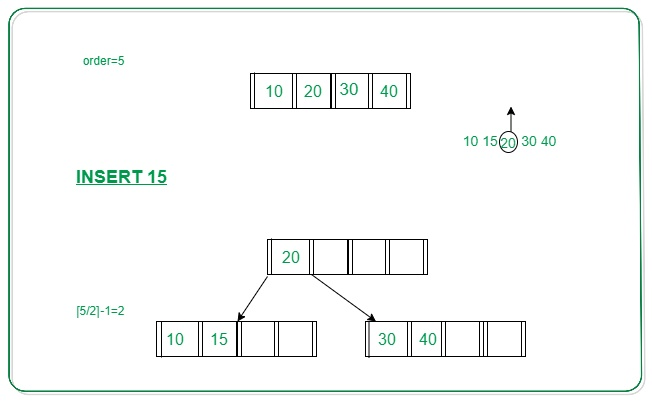
\includegraphics[scale=0.4]{in2.jpeg}
    \label{in2}
\end{figure}

\noindent \large {\textbf{Example to illustrate insertion on a B+ tree}} \vspace{0.5cm}

\noindent \textbf{Problem:} Insert the following key values 6, 16, 26, 36, 46 on a B+ tree with order = 3.

\noindent \textbf{Solution:} \vspace{2cm}

\noindent \textbf{Step 1:} The order is 3 so at maximum in a node so there can be only 2 search key values. As insertion happens on a leaf node only in a B+ tree so insert search key value 6 and 16 in increasing order in the node. Below is the illustration of the same:

\begin{figure}[h]
    \centering
    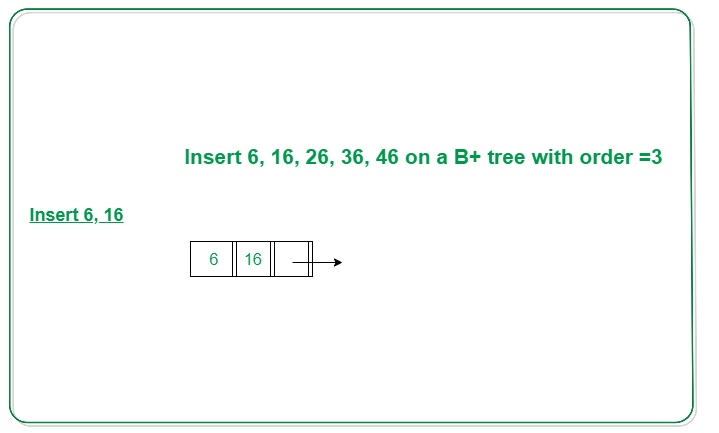
\includegraphics[scale=0.4]{in3.jpeg}
    \label{in3}
\end{figure}

\noindent \textbf{Step 2:} We cannot insert 26 in the same node as it causes an overflow in the leaf node, We have to split the leaf node according to the rules. First part contains ceil((3-1)/2) values i.e., only 6. The second node contains the remaining values i.e., 16 and 26. Then also copy the smallest search key value from the second node to the parent node i.e., 16 to the parent node. Below is the illustration of the same:

\begin{figure}[h]
    \centering
    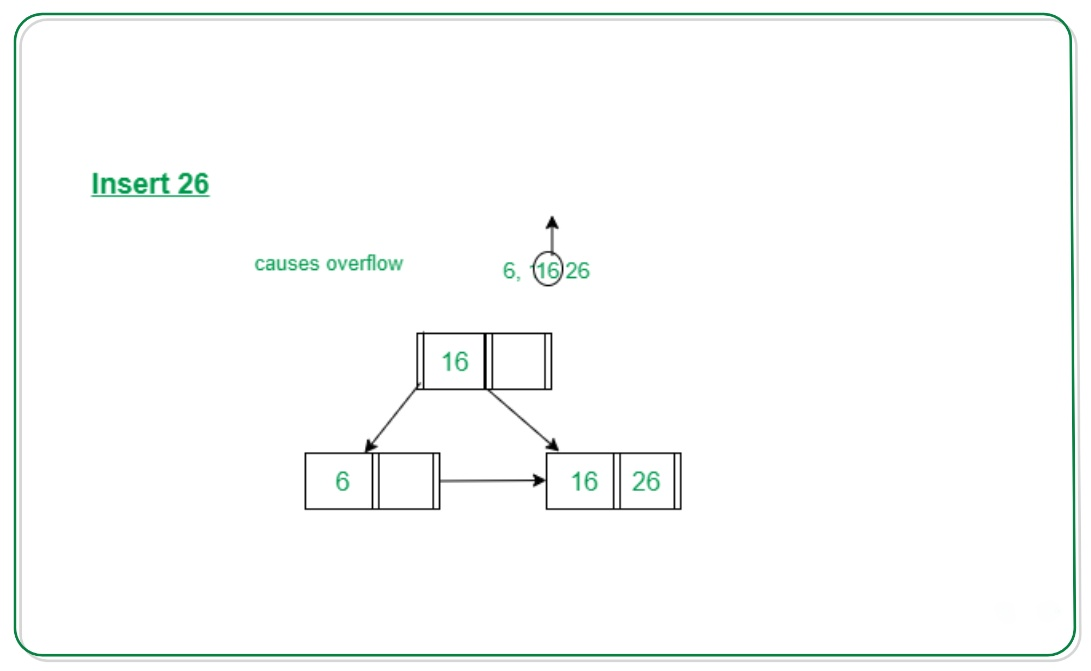
\includegraphics[scale=0.3]{in4.jpeg}
    \label{in4}
\end{figure}

\noindent \textbf{Step 3:} Now the next value is 36 that is to be inserted after 26 but in that node, it causes an overflow again in that leaf node. Again follow the above steps to split the node. First part contains ceil((3-1)/2) values i.e., only 16. The second node contains the remaining values i.e., 26 and 36. Then also copy the smallest search key value from the second node to the parent node i.e., 26 to the parent node. Below is the illustration of the same:
The illustration is shown in the diagram below. \vspace{4cm}

\begin{figure}[h]
    \centering
    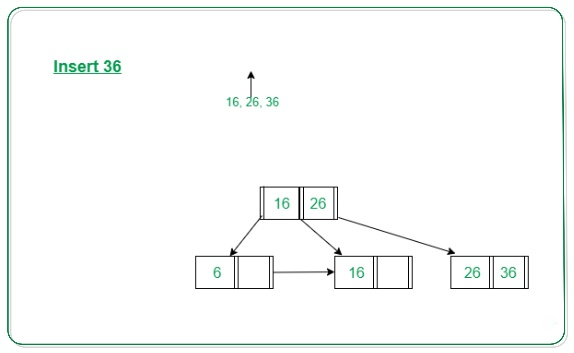
\includegraphics[scale=0.5]{in5.jpeg}
    \label{in5}
\end{figure}

\noindent \textbf{Step 4:} Now the next value is 36 that is to be inserted after 26 but in that node, it causes an overflow again in that leaf node. Again follow the above steps to split the node. First part contains ceil((3-1)/2) values i.e., only 16. The second node contains the remaining values i.e., 26 and 36. Then also copy the smallest search key value from the second node to the parent node i.e., 26 to the parent node. Below is the illustration of the same:
The illustration is shown in the diagram below.

\begin{figure}[h]
    \centering
    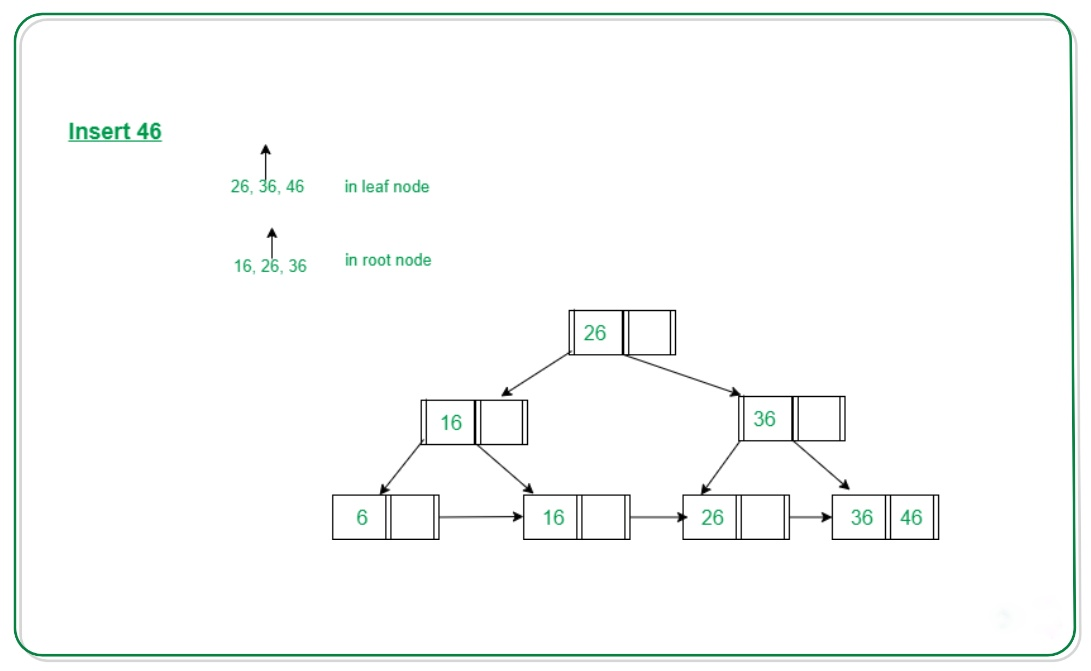
\includegraphics[scale=0.3]{in6.jpeg}
    \label{in6}
\end{figure}

\section{Complexity Analysis}
\begin{table}[h]
    \centering
    \caption{Time complexity in big O notation} \vspace{.2cm}
    \begin{tabular}{| c | c | c |}
    \hline
    \textbf{Algorithm} & \textbf{Average} & \textbf{Worst Case}\\
    \hline
    \textbf{Space} & O(n) & O(n) \\
    \hline
    \textbf{Search} & O(log n) & O(log n + log L) \\
    \hline
    \textbf{Insert} & O(log n) & O(M*log n + log L) \\
    \hline
    \textbf{Delete} & O(log n) & O(M*log n + log L)\\
    \hline
    \end{tabular}
    
    \label{tab:complexity}
\end{table}

\end{document}
